\documentclass[10pt,a4j,twocolumn]{jsarticle}
\usepackage[dvipdfmx]{graphicx}
%\usepackage[dvipdfmx]{hyperref}
\usepackage{url}
\usepackage{here}

\setlength{\textheight}{275mm}
\headheight 5mm
\topmargin -30mm
\textwidth 185mm
\oddsidemargin -15mm
\evensidemargin -15mm
\pagestyle{empty}

\begin{document}
\title{Githubを利用したRuby初心者学習ソフトの開発}
\author{関西学院大学 情報科学科 西谷研究室 2549 浦田 航貴}
\date{}
\maketitle
\section{目的}
プログラミング初心者は,初心者向けのテキストを使って言語の文法を習得する.しかし,プログラマーになるためには,ソフト開発に必要なその他の振舞い,テスト実行やバックアップ習慣を身につける必要がある.

本研究で開発するruby\_noviceは,Ruby言語の習得のみならず,周辺技能の習得を支援する環境提供を目指している.進捗管理やメンターからの添削をより容易におこなえるよう,バージョン管理ソフトGithubを利用したシステムを開発した.

\section{開発手法}
ruby\_noviceでは,学習者自身で書いたコードを開発現場で使用されている一般的なテスト環境でテストする.本研究でモデルとしたテスト駆動開発ならびに比較検討したフレームワークを下記に示す.
\subsection{TDD(Test Driven Development)}
プログラミング開発の最先端の技法としてTDDが奨励されている.TDDでは,仕様を満たすテストを書く(Red), テストを通るコードを書く(Green), コードを読みやすく直す(Refactoring)というステップでプログラミングを進めていくことを基本としている.それぞれの段階で次に作業する目標が明確になり,コード開発の効率が上がる.
\subsection{test::unit}
test::unitは,比較対象としたRuby用のxUnit 系の単体テストフレームワークである.Ruby1.8までは Ruby本体に標準添付されており,広く利用されている.
\subsection{aruba}
arubaは,Cucumber,RSpec,Minitestのような人気のあるTDD/BDD フレームワーク
で,コマンドラインアプリケーションのテストを簡単で楽しいものにする拡張である\cite{aruba}.

\section{開発ソフトの仕様}
本研究で開発したソフトruby\_noviceは,以下の3つの機能を有している.
\begin{enumerate}
\item Rubyの標準ライブラリ配布機構であるrubygemsに従っている
\item Githubを使って学習者のレポート提出機構を提供している
\item arubaにより学習者自身によるテスト機能を提供している
\end{enumerate}

%各章の概要は,以下の通りである.\\
%*第1章 (list1.1 〜 1.7):  putsメソッドやpメソッド\\
%*第3章 (list3.1 〜 3.11): ファイルの読み込み\\
%*第4章 (list4.1):        ローカル変数とグローバル変数\\
%*第5章 (list5.1 〜 5.5):  条件判断(if, unlessなど)\\
%*第6章 (list6.1 〜 6.13): 繰り返し(for,times,whileなど)\\
%*第7章 (list7.1 〜 7.4):  メソッド\\

ruby\_novice の構造は,図1のように3つに分かれている.
\begin{figure}[H]
\begin{center}
     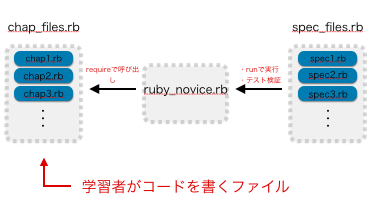
\includegraphics[width=9cm, bb=0 0 644 342]{abst.jpg}
     \caption{ruby\_noviceの構造.}
\end{center}
%\vspase{0\baselineskip}
\end{figure}

\begin{description}
\item[chap\_files.rb (chap1.rb ...)]Textのコードを書く部分.
\item[ruby\_novice.rb] chap\_files.rbを呼び出している.
\item[spec\_files.rb]出力結果 = 期待している値の検証.
\end{description}

現状は,「たのしいRuby」\cite{HappyRuby}の第1章〜第7章までのテストを実装している.テスト環境としては,環境変数RUBYNOVICE\_NAMEにディレクトリ名を入れるだけで,個人ごとにテストすることができる.また各章ごとや各問題ごとにテストができ,1問ずつ確認しながらコードを書いていくことが可能である.

\section{まとめ}
arubaは, print をそのまま出力でき,テストが可能である.また学習者がtextを見ながら書いていけるというメリットがある.これにより学習コストや些細なバグを削減できる.

今後の課題としては,現段階でtextの7章までしかテストコードを書けていないので引き続き書くことである.また問題にClassがあるコード(8章)は, 今まで通りコードを写すだけではテストできないので別のTDDフレームワークと比較して考える必要がある.


\begin{thebibliography}{9}
\bibitem{aruba}「Qiita Aruba gemでCLIのテストを支援する」, tbpgrさん, \url{http://qiita.com/tbpgr/items/41730edcdb07bb5b59ad}, 2017/2/12アクセス.
\bibitem{HappyRuby}「たのしいRuby」高橋 征義, 後藤 裕蔵, まつもと ゆきひろ (監)(SBクリエイティブ,2016).
\end{thebibliography}

\end{document}